\documentclass[11pt]{amsart}
\usepackage[T1]{fontenc}
\usepackage{iftex}
\ifPDFTeX\usepackage[utf8]{inputenc}\fi
\usepackage{lmodern}
\usepackage[margin=1.05in]{geometry}
\usepackage{amssymb,mathtools,booktabs,array,graphicx}
\usepackage[hidelinks]{hyperref}
\hypersetup{pdftitle={A homogeneous mono-unstable polyhedron with fourteen vertices},pdfauthor={Claudio Mattioni}}
\newtheorem{theorem}{Theorem}
\newtheorem{lemma}{Lemma}
\newtheorem{corollary}{Corollary}
\theoremstyle{remark}
\newtheorem*{remark}{Remark}
\newcommand{\R}{\mathbb R}
\newcommand{\conv}{\operatorname{conv}}
\newcommand{\vol}{\operatorname{vol}}
\newcommand{\sgn}{\operatorname{sgn}}
\urlstyle{same}
\title[A mono-unstable polyhedron with fourteen vertices]{A homogeneous mono-unstable polyhedron\\with fourteen vertices}
\author{Claudio Mattioni}
\email{claudio.mattioni@gmail.com}
\date{November 17, 2026. Version 1.0. Preprint, not peer reviewed.}

\begin{document}
\begin{abstract}
We give an explicit convex polyhedron with fourteen vertices whose uniformly distributed volume has exactly one unstable equilibrium with respect to its center of mass. The vertices have small integer coordinates, and the polyhedron has twenty-four triangular facets. Its equilibrium counts are two stable, one unstable, and one saddle equilibrium. The construction controls the projected center of mass by varying the thickness along a double-spiral outline, without introducing an additional apex. We provide a self-contained exact verification using integer arithmetic. We also prove that every positive vertical contraction of the example remains mono-unstable, giving an explicit one-parameter family with the same fourteen-vertex face lattice.
\end{abstract}
\maketitle

\section{Introduction}\label{sec:intro}

Let $P\subset\R^3$ be a full-dimensional convex polyhedron with uniform volume density and center of mass $c$. A boundary point $q$ is an equilibrium if the plane through $q$ perpendicular to $q-c$ supports $P$. The equilibrium is nondegenerate when that plane meets $P$ exactly in the face whose relative interior contains $q$. Such an equilibrium is stable, of saddle type, or unstable when that face has dimension two, one, or zero, respectively. We denote the respective counts by $S,H,U$. A polyhedron is \emph{mono-unstable} if $U=1$.

The construction problem asks how few vertices a homogeneous convex polyhedron with a unique unstable equilibrium can have. The reference point is its actual volume centroid; replacing it by the average of the vertices changes the problem. In particular, the minimum of eleven vertices established for equal point masses at the vertices~\cite{PRDB23} does not apply to the uniformly filled solid considered here.

Domokos, Kov\'acs, L\'angi, Reg\H{o}s and Varga~\cite[Section~4.2]{DKLRV20} constructed mono-unstable pyramids with eighteen vertices. Their example $P_2$ has $S=2,H=1,U=1$. Reg\H{o}s~\cite{Reg25} subsequently supplied integer-coordinate realizations of earlier monostatic constructions. A public repository dated July~13, 2026~\cite{Public16} supplies a mono-unstable pyramid with sixteen vertices and sixteen facets. We include this public construction in the comparison even though the source is a repository rather than a journal article.

The present construction uses fourteen vertices and no extra apex. Table~\ref{tab:comparison} records the tradeoff: the number of vertices decreases, whereas the numbers of edges and facets increase. Thus the result is an upper bound for the minimum number of vertices, not a simultaneous improvement in every size measure.

\begin{table}[ht]
\centering
\caption{Explicit homogeneous examples with $S=2,H=1,U=1$. The last column is the mechanical complexity of~\cite{DKLRV20}.}\label{tab:comparison}
\begin{tabular}{lrrrr}
\toprule
Construction & $V$ & $E$ & $F$ & $V+E+F-S-H-U$\\
\midrule
$P_2$ of~\cite{DKLRV20} & 18 & 34 & 18 & 66\\
Public construction~\cite{Public16} & 16 & 30 & 16 & 58\\
This paper & 14 & 36 & 24 & 70\\
\bottomrule
\end{tabular}
\end{table}

The vertex lower-bound problem has a different character. Boz\'oki, Domokos, Papp and Reg\H{o}s~\cite{BDPR24} prove a lower bound of seven vertices using exact infeasibility certificates. A recent public research archive~\cite{Hum26} proposes stronger lower bounds and contains numerous construction reports. We do not use any of those proposed bounds in the proof below. The assertion proved here is the constructive bound $V_U\le14$.

The fourteen-facet mono-stable polyhedron of Reshetov~\cite{Res14} addresses the face version of the problem. Polarity exchanges stable faces and unstable vertices with respect to a fixed interior reference point, but it does not in general preserve the volume centroid. Consequently, polarizing that example does not by itself give the homogeneous mono-unstable construction required here.

\begin{theorem}\label{thm:main}
The convex hull of the fourteen integer points in Table~\ref{tab:points}, with uniform volume density, has fourteen vertices, thirty-six edges and twenty-four triangular facets. Its unique unstable equilibrium is vertex $0$. It has exactly two stable equilibria, on facets $\{0,5,7\}$ and $\{0,6,13\}$, and one saddle equilibrium, on edge $\{6,7\}$; all its equilibria are nondegenerate.
\end{theorem}

\begin{corollary}\label{cor:family}
Write the points of Table~\ref{tab:points} as $p_i=(x_i,y_i,z_i)$. For every $0<t\le1$, the uniformly filled polyhedron
\[
 P_t=\conv\{(x_i,y_i,tz_i):0\le i\le13\}
\]
has the same fourteen-vertex face lattice and exactly one unstable equilibrium.
\end{corollary}

The corollary concerns $U=1$ throughout the interval. The full count $S=2,H=1,U=1$ in Theorem~\ref{thm:main} is asserted for the tabulated example, $t=1$. We neither claim that fourteen is minimal nor exclude constructions with thirteen or fewer vertices.

\section{Geometric mechanism}\label{sec:mechanism}

\subsection{A spiral outline and a movable center of mass}
A useful starting point is a planar chain about a reference point $O$. If successive ray angles are $\varphi_k$ and the radii satisfy
\[
 r_k=r_{k-1}\cos\varphi_k,
\]
then $(P_{k-1}-P_k)\cdot(P_k-O)=0$. Moving the reference point to $O+\delta$ makes this product positive whenever
$\delta\cdot(P_{k-1}-P_k)<0$. Two arms arranged on either side of their common endpoint can therefore provide a sequence of strict escape directions toward that endpoint.

The difficulty is to place the actual centroid in the required region. The spiral construction and the use of three-dimensional geometry to move a projected centroid have classical precedents; in particular, the pyramids in~\cite[Section~4.2]{DKLRV20} use an apex near one end of the planar outline. Our construction gives small heights directly to the outline vertices. These heights alternate near the lower part of the outline, producing more volume there without adding an apex. Numerical searches within this family produced examples that could be rounded to the small integers in Table~\ref{tab:points}. The proof uses those integers alone and does not depend on the optimizer or its tolerances.

\begin{figure}[ht]
\centering
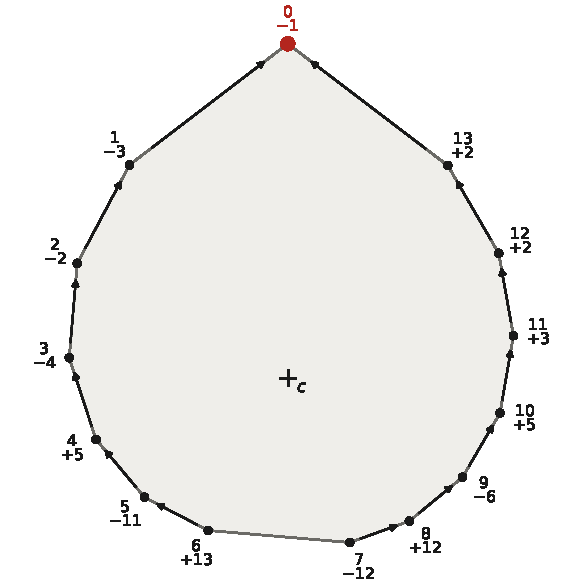
\includegraphics[width=0.53\textwidth]{V14_plate.pdf}
\caption{Projection onto the $(x,y)$-plane. Each label gives a vertex index and its signed height $z_i$. Arrows are the exact escape witnesses $i\to j$ used below. The cross marks the projected volume centroid; the highlighted point is the unique unstable vertex. This is an orthogonal projection, not a three-dimensional drawing to scale.}\label{fig:plate}
\end{figure}

\subsection{Thickness and vertical contraction}
More generally, let $p_i=(q_i,h_i)$, with $q_i\in\R^2$, and let $P_1=\conv\{p_i\}$. Over its projected outline $K$, write the upper and lower boundary heights as $u(q)$ and $\ell(q)$. The thickness is
$w(q)=u(q)-\ell(q)$. Fubini's theorem gives the projected volume centroid
\begin{equation}\label{eq:thickness}
 c'=\frac{\int_K q\,w(q)\,dq}{\int_K w(q)\,dq}.
\end{equation}
The density in space is constant. The nonuniform weight in~\eqref{eq:thickness} is the amount of material above each projected point, not an imposed material density.

Under the invertible map $L_t=\operatorname{diag}(1,1,t)$, $t>0$, the centroid is $c_t=L_tc=(c',tc_z)$. For any two vertices,
\begin{equation}\label{eq:flatten}
 (L_tp_j-L_tp_i)\cdot(L_tp_i-c_t)
 =(q_j-q_i)\cdot(q_i-c')+t^2(h_j-h_i)(h_i-c_z).
\end{equation}
Thus heights can shape the projected mass distribution while their direct contribution to the escape inequalities decreases quadratically as the body is flattened. If all but one vertex have strictly positive planar escape witnesses, sufficiently small positive $t$ preserves those witnesses. The remaining vertex must be unstable: a vertex farthest from the interior point $c_t$ has a strictly supporting perpendicular plane. Section~\ref{sec:family} gives an explicit interval for the particular example.

\section{Exact construction and proof}\label{sec:proof}

\subsection{Coordinates and convex hull}
\begin{table}[ht]
\centering
\caption{The fourteen vertices. All coordinates are integers.}\label{tab:points}
\begin{tabular}{rrrr@{\qquad}rrrr}
\toprule
$i$ & $x_i$ & $y_i$ & $z_i$ & $i$ & $x_i$ & $y_i$ & $z_i$\\
\midrule
0 & -4 & 1000 & -1 & 7 & 181 & -490 & -12\\
1 & -477 & 638 & -3 & 8 & 359 & -426 & 12\\
2 & -633 & 344 & -2 & 9 & 518 & -295 & -6\\
3 & -657 & 62 & -4 & 10 & 630 & -103 & 5\\
4 & -577 & -182 & 5 & 11 & 670 & 128 & 3\\
5 & -432 & -355 & -11 & 12 & 626 & 374 & 2\\
6 & -242 & -454 & 13 & 13 & 474 & 636 & 2\\
\bottomrule
\end{tabular}
\end{table}

The outward-oriented facet triples, in the numbering of Table~\ref{tab:points}, are
\begin{equation}\label{eq:facets}
\begin{gathered}
(1,0,5),\ (1,6,0),\ (5,0,7),\ (6,13,0),\ (0,9,7),\ (0,13,9),\\
(3,2,1),\ (2,4,1),\ (3,1,5),\ (4,6,1),\ (3,4,2),\ (3,5,4),\\
(4,5,6),\ (5,7,6),\ (6,7,8),\ (6,8,13),\ (7,9,8),\ (8,9,10),\\
(8,10,11),\ (8,11,12),\ (8,12,13),\ (9,11,10),\ (9,12,11),\ (13,12,9).
\end{gathered}
\end{equation}
For each listed triple $(a,b,d)$, direct integer evaluation gives
\begin{equation}\label{eq:support}
 ((p_b-p_a)\times(p_d-p_a))\cdot(p_k-p_a)<0
 \quad\text{for every }k\notin\{a,b,d\}.
\end{equation}
There are $24\cdot11=264$ such tests. Each triangle is consequently an exposed facet, and every listed point is a vertex. Each of the thirty-six undirected edges occurs in exactly two triangles, with opposite orientations. This proves completeness of the facet list: the listed facets form a nonempty subset closed under passage to an adjacent facet across an edge, and the facet adjacency graph of a convex polyhedron is connected. In particular, the hull has the stated $f$-vector. Strict support also certifies full dimension.

\subsection{Volume and centroid}
For an outward-oriented triangle with position vectors $a,b,d$, let $\det(a,b,d)=a\cdot(b\times d)$. Signed tetrahedral integration gives
\begin{equation}\label{eq:mass}
 D=\sum\det(a,b,d)=6\vol(P),\qquad
 C=\sum\det(a,b,d)(a+b+d)=24\vol(P)c.
\end{equation}
These signed sums are valid even when the origin is outside a constituent tetrahedron. Applying~\eqref{eq:mass} to~\eqref{eq:facets} yields
\[
 D=90\,438\,831,\qquad
 C=(-948\,565\,765,\ 351\,349\,436,\ 24\,043\,586).
\]
Hence $\vol(P)=30\,146\,277/2$, $W:=4D=361\,755\,324$, and
\begin{equation}\label{eq:centroid}
 c=C/W
 =\left(-\frac{135509395}{51679332},
          \frac{87837359}{90438831},
          \frac{1717399}{25839666}\right).
\end{equation}
The integer vectors $g_i=Wp_i-C=W(p_i-c)$ allow the remaining tests to be performed without rational division.

\subsection{The unique unstable equilibrium}
\begin{lemma}\label{lem:vertex}
A vertex $p_i$ of a convex polyhedron containing $c$ in its interior is a nondegenerate unstable equilibrium if and only if
\[
 (p_j-p_i)\cdot(p_i-c)<0
\]
for every neighbor $p_j$ of $p_i$. A single strictly positive value, even for a nonadjacent vertex, excludes an equilibrium at $p_i$.
\end{lemma}
\begin{proof}
The edge directions at $p_i$ generate its tangent cone. If the displayed scalar products are all negative, their nonzero nonnegative combinations are negative, so the plane through $p_i$ normal to $p_i-c$ meets the hull only at $p_i$. Conversely, a strictly supporting plane gives the inequalities on every edge. A positive value places another point on the opposite side of the plane from $c$, so the plane is not supporting.
\end{proof}

Set
\[
 s(i,j)=(p_j-p_i)\cdot g_i.
\]
Table~\ref{tab:witnesses} lists a neighbor $j$ with $s(i,j)>0$ for every $i\ne0$. The six neighbors of vertex $0$ are $1,5,6,7,9,13$; exact evaluation gives
\[
 \max_{j\sim0}s(0,j)=-130\,591\,697\,728\,185<0.
\]
Lemma~\ref{lem:vertex} therefore proves that vertex $0$ is the sole unstable equilibrium, with no degenerate vertex equilibria.

\begin{table}[ht]
\centering
\caption{Exact escape witnesses and coefficients used for the contraction family. The last column equals $A_{ij}+B_{ij}=s(i,j)$.}\label{tab:witnesses}
\small
\begin{tabular}{rrrrr}
\toprule
$i$ & $j$ & $A_{ij}$ & $B_{ij}$ & $s(i,j)$\\
\midrule
1 & 0 & 2251447764553 & -2218619116 & 2249229145437\\
2 & 1 & 908551238868 & 747554234 & 909298793102\\
3 & 2 & 544457173392 & -2942129764 & 541515043628\\
4 & 3 & 472180804064 & -16062597306 & 456118206758\\
5 & 4 & 244824783547 & -64053634400 & 180771149147\\
6 & 5 & 159043915502 & -112290615024 & 46753300478\\
7 & 8 & 456744410258 & -104762579376 & 351981830882\\
8 & 9 & 566033218619 & -77706365436 & 488326853183\\
9 & 10 & 536555599792 & -24140330830 & 512415268962\\
10 & 11 & 465770651752 & -3569466068 & 462201185684\\
11 & 12 & 598235835676 & -1061222386 & 597174613290\\
12 & 13 & 789702550352 & 0 & 789702550352\\
13 & 0 & 1202871627594 & -2098401186 & 1200773226408\\
\bottomrule
\end{tabular}
\end{table}

\subsection{Stable and saddle equilibria}\label{sec:census}
For completeness, we give the predicates used to classify all facets and all true edges. These also give a direct finite verification of the additional equilibrium counts in Theorem~\ref{thm:main}.

For an outward-oriented facet $(a,b,d)$, put
\[
 n=(p_b-p_a)\times(p_d-p_a),\quad N=n\cdot n,\quad
 h=n\cdot(p_a-c),\quad q=c+(h/N)n.
\]
The facet is stable exactly when the following three quantities are positive, with $(i,j)$ running cyclically through $(a,b),(b,d),(d,a)$:
\begin{equation}\label{eq:facepredicate}
 n\cdot\big((p_j-p_i)\times(q-p_i)\big).
\end{equation}
The common denominator can be cleared by using $WNq=NC+(Wn\cdot p_a-n\cdot C)n$.

For an edge $\{a,b\}$, put
\[
 e=p_b-p_a,\qquad
 \tau=\frac{e\cdot(c-p_a)}{e\cdot e},\qquad q=p_a+\tau e.
\]
It carries a nondegenerate saddle exactly when
\begin{equation}\label{eq:edgepredicate}
 0<\tau<1,\qquad (p_k-p_a)\cdot(q-c)<0
 \quad(k\notin\{a,b\}).
\end{equation}
The first pair puts $q$ inside the segment. The other inequalities make its perpendicular plane strictly supporting away from that edge. These are global support tests, so no inference from Euler or the equilibrium index formula is needed.

Evaluating~\eqref{eq:facepredicate} over the twenty-four facets gives positive triples only for $\{0,5,7\}$ and $\{0,6,13\}$. Every other facet has a strictly negative predicate. Evaluating~\eqref{eq:edgepredicate} over the thirty-six edges gives a saddle only for $\{6,7\}$; every other edge violates at least one condition strictly. The complete sign ledger is supplied in Appendix~\ref{app:ledger}, and the exact integer numerators are in \path{examples/V14_family_report.json}. There are no degenerate face or edge equilibria. Together with the vertex calculation, this completes the proof of Theorem~\ref{thm:main}. The identity $S-H+U=2$ is an additional consistency check.

\section{An explicit interval of contractions}\label{sec:family}

For the coordinates in Table~\ref{tab:points}, define
\begin{align*}
 A_{ij}&=(x_j-x_i)(Wx_i-C_x)+(y_j-y_i)(Wy_i-C_y),\\
 B_{ij}&=(z_j-z_i)(Wz_i-C_z).
\end{align*}
Multiplying~\eqref{eq:flatten} by $W$ gives $A_{ij}+t^2B_{ij}$. Table~\ref{tab:witnesses} shows that both $A_{ij}$ and $A_{ij}+B_{ij}$ are strictly positive for all thirteen chosen witnesses. For $0\le t^2\le1$,
\[
 A_{ij}+t^2B_{ij}=(1-t^2)A_{ij}+t^2(A_{ij}+B_{ij})>0.
\]
The map $L_t$ is invertible for $t>0$, so it preserves the face lattice and all chosen witness edges. Consequently every vertex except $0$ remains strictly non-equilibrium.

To see that the remaining vertex is unstable, choose a vertex $v$ of maximal distance from $c_t$. For any other vertex $w$, the Cauchy--Schwarz inequality gives
\[
 (w-v)\cdot(v-c_t)
 \le |w-c_t|\,|v-c_t|-|v-c_t|^2\le0.
\]
Equality would require $w-c_t=v-c_t$, contrary to distinctness. Thus some vertex is strictly unstable, and the escape witnesses force it to be vertex $0$. This proves Corollary~\ref{cor:family}. The independent checker also directly verifies negative support signs at vertex $0$ throughout the interval.

\begin{remark}
The zero-thickness limit is excluded: $P_0$ is planar. For each positive $t$ the body has positive volume and uniform spatial density. The argument supplies an interval of mono-instability, not a proof that its endpoint $t=1$ is maximal.
\end{remark}

\section{Verification, scope and reproducibility}\label{sec:verification}

The central existence proof consists of the explicit coordinates and the finite integer calculations in Section~\ref{sec:proof}. The coefficient table then proves an infinite family without numerical sampling in $t$. No search program or floating-point tolerance is part of these proofs.

The accompanying archive contains three complementary checking paths:
\begin{enumerate}
\item \path{examples/V14_short_check.py} checks the supplied supporting triangles, closure of their edge incidences, signed volume and centroid, and the thirteen escape witnesses. This short program certifies $U=1$.
\item \path{verify/exact_verify.py} independently reconstructs the convex hull and classifies all equilibria using exact rational arithmetic.
\item \path{verify/check_c.py} reconstructs the triangular hull by exhaustive point triples, checks face and edge feet by global integer support tests, and verifies the contraction interval. It does not import either of the other checkers.
\end{enumerate}
All three verification paths use only the Python standard library. The command
\begin{verbatim}
python reproduce.py
\end{verbatim}
checks the integrity manifest, runs the verifiers, and compares regenerated exact reports and manuscript tables with the supplied data. It does not require a virtual environment, an optimizer, or a network connection. The package includes a transcript of an execution from an extracted copy.

The construction improves the explicit vertex count to fourteen among the sources compared here. It does not prove optimality, a lower bound for thin plates, a mono-stable example with fewer facets, or the existence of a polyhedral G\"omb\"oc: the tabulated body has two stable equilibria. Whether a homogeneous convex mono-unstable polyhedron with at most thirteen vertices exists remains open in this work.

\subsection*{Use of AI}
The original searches, code and draft were developed with substantial assistance from Claude (Anthropic), directed by the author. The present restructuring, literature comparison, additional exact checker and contraction certificate were prepared with assistance from Codex (OpenAI). Computational checks by AI-assisted implementations are not human peer review. No external human expert review is claimed.

\subsection*{Data availability and licences}
The accompanying package supplies this manuscript, its LaTeX and Markdown sources, exact coordinates, verification programs, reports, figure source and reproduction instructions. Its associated Zenodo DOI is
\href{https://doi.org/10.5281/zenodo.24286668}{10.5281/zenodo.24286668}.
The DOI was reserved during preparation; the record remained a draft while this version was assembled. Code is licensed under MIT; the manuscript, figures, data and documentation under CC BY 4.0. The file-type rule and full licence texts are included.

\appendix
\section{Complete equilibrium sign ledger}\label{app:ledger}
The tables below are generated from the integer predicates of Section~\ref{sec:census}. For each oriented facet, the three signs follow its cyclic edge order. A facet is stable only for $+++$. For an edge, the first two signs belong to $\tau$ and $1-\tau$; a support sign $+$ means the corresponding strict inequality in~\eqref{eq:edgepredicate} holds. The twelve support signs are listed in increasing vertex order, omitting the edge endpoints. Every rejected feature has a minus sign. The machine-readable report includes every unreduced integer numerator, so the signs can be recomputed from the coordinate table without trusting this ledger.
% Generated by make_ledger.py; integer signs only.
\begin{table}[ht]
\centering\small
\caption{Facet predicates in cyclic order. Exactly two rows have three plus signs.}\label{tab:faceledger}
\begin{tabular}{lc@{\qquad\qquad}lc}
\toprule
Oriented facet & Signs & Oriented facet & Signs\\
\midrule
$(0,5,1)$ & \texttt{-++} & $(4,5,6)$ & \texttt{++-}\\
$(0,1,6)$ & \texttt{++-} & $(5,7,6)$ & \texttt{-++}\\
$(0,7,5)$ & \texttt{+++} & $(6,7,8)$ & \texttt{++-}\\
$(0,6,13)$ & \texttt{+++} & $(6,8,13)$ & \texttt{++-}\\
$(0,9,7)$ & \texttt{++-} & $(7,9,8)$ & \texttt{-++}\\
$(0,13,9)$ & \texttt{++-} & $(8,9,10)$ & \texttt{++-}\\
$(1,3,2)$ & \texttt{-++} & $(8,10,11)$ & \texttt{++-}\\
$(1,2,4)$ & \texttt{++-} & $(8,11,12)$ & \texttt{++-}\\
$(1,5,3)$ & \texttt{-++} & $(8,12,13)$ & \texttt{++-}\\
$(1,4,6)$ & \texttt{++-} & $(9,11,10)$ & \texttt{-++}\\
$(2,3,4)$ & \texttt{++-} & $(9,12,11)$ & \texttt{-++}\\
$(3,5,4)$ & \texttt{-++} & $(9,13,12)$ & \texttt{-++}\\
\bottomrule
\end{tabular}
\end{table}
\clearpage

\begin{table}[ht]
\centering\footnotesize
\caption{Edge predicates: two segment signs and twelve global support signs. Only edge $\{6,7\}$ has all positive signs.}\label{tab:edgeledger}
\begin{tabular}{lcc@{\qquad}lcc}
\toprule
Edge & Segment & Support & Edge & Segment & Support\\
\midrule
$\{0,1\}$ & \texttt{+-} & \texttt{++++++++++++} & $\{5,7\}$ & \texttt{++} & \texttt{+++++-++++++}\\
$\{0,5\}$ & \texttt{++} & \texttt{----++++++++} & $\{6,7\}$ & \texttt{++} & \texttt{++++++++++++}\\
$\{0,6\}$ & \texttt{++} & \texttt{-----+++++++} & $\{6,8\}$ & \texttt{++} & \texttt{++++++-+++++}\\
$\{0,7\}$ & \texttt{++} & \texttt{++++++------} & $\{6,13\}$ & \texttt{++} & \texttt{++++++------}\\
$\{0,9\}$ & \texttt{++} & \texttt{++++++++----} & $\{7,8\}$ & \texttt{-+} & \texttt{++++++++++++}\\
$\{0,13\}$ & \texttt{+-} & \texttt{++++++++++++} & $\{7,9\}$ & \texttt{++} & \texttt{+++++++-++++}\\
$\{1,2\}$ & \texttt{+-} & \texttt{++++++++++++} & $\{8,9\}$ & \texttt{-+} & \texttt{++++++++++++}\\
$\{1,3\}$ & \texttt{++} & \texttt{+-++++++++++} & $\{8,10\}$ & \texttt{++} & \texttt{++++++++-+++}\\
$\{1,4\}$ & \texttt{++} & \texttt{+--+++++++++} & $\{8,11\}$ & \texttt{++} & \texttt{++++++++--++}\\
$\{1,5\}$ & \texttt{++} & \texttt{+---++++++++} & $\{8,12\}$ & \texttt{++} & \texttt{++++++++---+}\\
$\{1,6\}$ & \texttt{++} & \texttt{+----+++++++} & $\{8,13\}$ & \texttt{++} & \texttt{++++++++----}\\
$\{2,3\}$ & \texttt{+-} & \texttt{++++++++++++} & $\{9,10\}$ & \texttt{-+} & \texttt{++++++++++++}\\
$\{2,4\}$ & \texttt{++} & \texttt{++-+++++++++} & $\{9,11\}$ & \texttt{++} & \texttt{+++++++++-++}\\
$\{3,4\}$ & \texttt{+-} & \texttt{++++++++++++} & $\{9,12\}$ & \texttt{++} & \texttt{+++++++++--+}\\
$\{3,5\}$ & \texttt{++} & \texttt{+++-++++++++} & $\{9,13\}$ & \texttt{++} & \texttt{+++++++++---}\\
$\{4,5\}$ & \texttt{+-} & \texttt{++++++++++++} & $\{10,11\}$ & \texttt{-+} & \texttt{++++++++++++}\\
$\{4,6\}$ & \texttt{++} & \texttt{++++-+++++++} & $\{11,12\}$ & \texttt{-+} & \texttt{++++++++++++}\\
$\{5,6\}$ & \texttt{+-} & \texttt{++++++++++++} & $\{12,13\}$ & \texttt{-+} & \texttt{++++++++++++}\\
\bottomrule
\end{tabular}
\end{table}


\begin{thebibliography}{10}

\bibitem{DKLRV20}
G.~Domokos, F.~Kov\'acs, Z.~L\'angi, K.~Reg\H{o}s and P.~T.~Varga,
\emph{Balancing polyhedra},
Ars Math. Contemp. \textbf{19} (2020), 95--124.
\href{https://arxiv.org/abs/1810.05382v3}{arXiv:1810.05382v3}.

\bibitem{Reg25}
K.~Reg\H{o}s, \emph{Homogeneous, Monostatic Lattice Polyhedra, or the Magic Pyramid with 17 Sides},
\'Ep\'it\'es--\'Ep\'it\'eszettudom\'any \textbf{53} (2025), no.~3--4, 203--217.
\href{https://doi.org/10.1556/096.2025.00142}{doi:10.1556/096.2025.00142}.

\bibitem{Public16}
GitHub user \texttt{shuhualin1023},
\emph{A mono-unstable homogeneous convex polyhedron with 16 faces and 16 vertices},
public repository \texttt{mono-unstable-16}, July~13, 2026.
\href{https://github.com/shuhualin1023/mono-unstable-16/tree/cf21399a241e48a1ca872b20846be46f6a7b8025}{Snapshot cf21399a241e48a1ca872b20846be46f6a7b8025}.
Accessed November~17, 2026.

\bibitem{BDPR24}
S.~Boz\'oki, G.~Domokos, D.~Papp and K.~Reg\H{o}s,
\emph{The smallest mono-unstable, homogeneous convex polyhedron has at least 7 vertices},
\href{https://arxiv.org/abs/2401.17906}{arXiv:2401.17906} (2024).

\bibitem{PRDB23}
D.~Papp, K.~Reg\H{o}s, G.~Domokos and S.~Boz\'oki,
\emph{The smallest mono-unstable convex polyhedron with point masses has 8 faces and 11 vertices},
European J. Oper. Res. \textbf{310} (2023), 511--517.
\href{https://doi.org/10.1016/j.ejor.2023.04.028}{doi:10.1016/j.ejor.2023.04.028}.

\bibitem{Res14}
A.~Reshetov, \emph{A unistable polyhedron with 14 faces},
Int. J. Comput. Geom. Appl. \textbf{24} (2014), 39--59.
\href{https://doi.org/10.1142/S0218195914500022}{doi:10.1142/S0218195914500022}.

\bibitem{Hum26}
O.~Humeniuk, \emph{Gomboc research},
public research archive, release \texttt{research-2026-10-12.3}, October~12, 2026.
\href{https://github.com/ohresearchresults/gomboc-research/releases/tag/research-2026-10-12.3}{GitHub release}.
Consulted at commit \texttt{0ec0d2569bd2b13c57b3bc6c7cad89882f7301b1};
see \href{https://github.com/ohresearchresults/gomboc-research/blob/0ec0d2569bd2b13c57b3bc6c7cad89882f7301b1/catalog/coverage.md}{verification status}, and
\href{https://github.com/ohresearchresults/gomboc-research/blob/0ec0d2569bd2b13c57b3bc6c7cad89882f7301b1/reports/minimum/minimum-0006.md}{report minimum-0006}.
Accessed November~17, 2026.

\end{thebibliography}
\end{document}
